\documentclass[12pt, a4paper, titlepage]{article}

% Cadenas traducidas al español.
\usepackage[spanish, es-tabla,es-noquoting,es-noshorthands]{babel}

% Para poder poner acentos, ñ's y similares en el documento.
\usepackage[T1]{fontenc}
\usepackage[utf8x]{inputenc}

% Paquetes para matemáticas
\usepackage{amsthm}
\usepackage{amsmath}
\usepackage{amssymb}

\usepackage{xcolor} 	% Colores
\usepackage{graphicx} 	% Imágenes
\usepackage{hyperref} 	% Enlaces
\usepackage{listings}   % Ejemplos de código
\usepackage{caption} 	% Para personalizar los "caption"
\usepackage{booktabs} 	% Para líneas (\hline) de tablas un poco mejores. Ver última sección.
\usepackage{fancyhdr} 	% Para la cabecera del documento

% Márgenes del documento
\usepackage[left = 3cm, right = 3cm, top = 3cm, bottom = 2cm]{geometry}

% Formato de los enlaces
\hypersetup{
	hyperindex,
	colorlinks,
	allcolors = blue!50!black
}

% Formato para las muestras de código
\lstset{
  basicstyle=\ttfamily\footnotesize,
  breaklines=true,
  commentstyle=\color{gray},
  stringstyle=\color{green!70!white},
  keywordstyle=\color{red!70!black},
  language=C
}

% Cambiando a un tipo de letra algo más interesante
\renewcommand*{\familydefault}{bch}
% Otras posibilidades en lugar de bch: ppl, pbk, cmr.
% Ver https://www.sharelatex.com/learn/Font_typefaces para una
% 	lista algo más extensa con muestras.

% Arreglando los captions:
\captionsetup{
	font = small, 	% Reducimos el tamaño de letra
	labelfont = bf	% Y además hacemos que el "Figura X" esté en negrita.
}

% Cabecera del documento
\fancyhf{}
\fancypagestyle{plain}{%
	\lhead{\itshape Práctica N} 	% lhead: cabecera, parte izquierda
	\rhead{Autores} 				% rhead: cabecera, parte derecha
	\cfoot{\thepage} 				% cfoot: pie, parte central
	\lfoot{\tiny\textsc{\today}} 	% chead: pie, parte izquierda
}


\author{Autores}
\date{\today}
\title{Ejemplo de memoria de prácticas \\ {\large\textsc{Asignatura}}}

\begin{document}
\maketitle

\pagestyle{plain} % Activamos las cabeceras de fancypagestyle

\tableofcontents
\newpage

\section{Ejercicio 1}

Se nos pide la implementación del algoritmo \textit{QuickSort} en C.

\subsection{Código fuente}

\begin{lstlisting}
// Quick sort function
void quick_sort (int *a, int n) {
    int i, j, p, t;
    if (n < 2)
        return;
    p = a[n / 2];
    for (i = 0, j = n - 1;; i++, j--) {
        while (a[i] < p)
            i++;
        while (p < a[j])
            j--;
        if (i >= j)
            break;
        t = a[i];
        a[i] = a[j];
        a[j] = t;
    }
    quick_sort(a, i);
    quick_sort(a + i, n - i);
}
\end{lstlisting}


\subsection{Resultados y rendimiento}

\begin{figure}[hbtp]
\centering
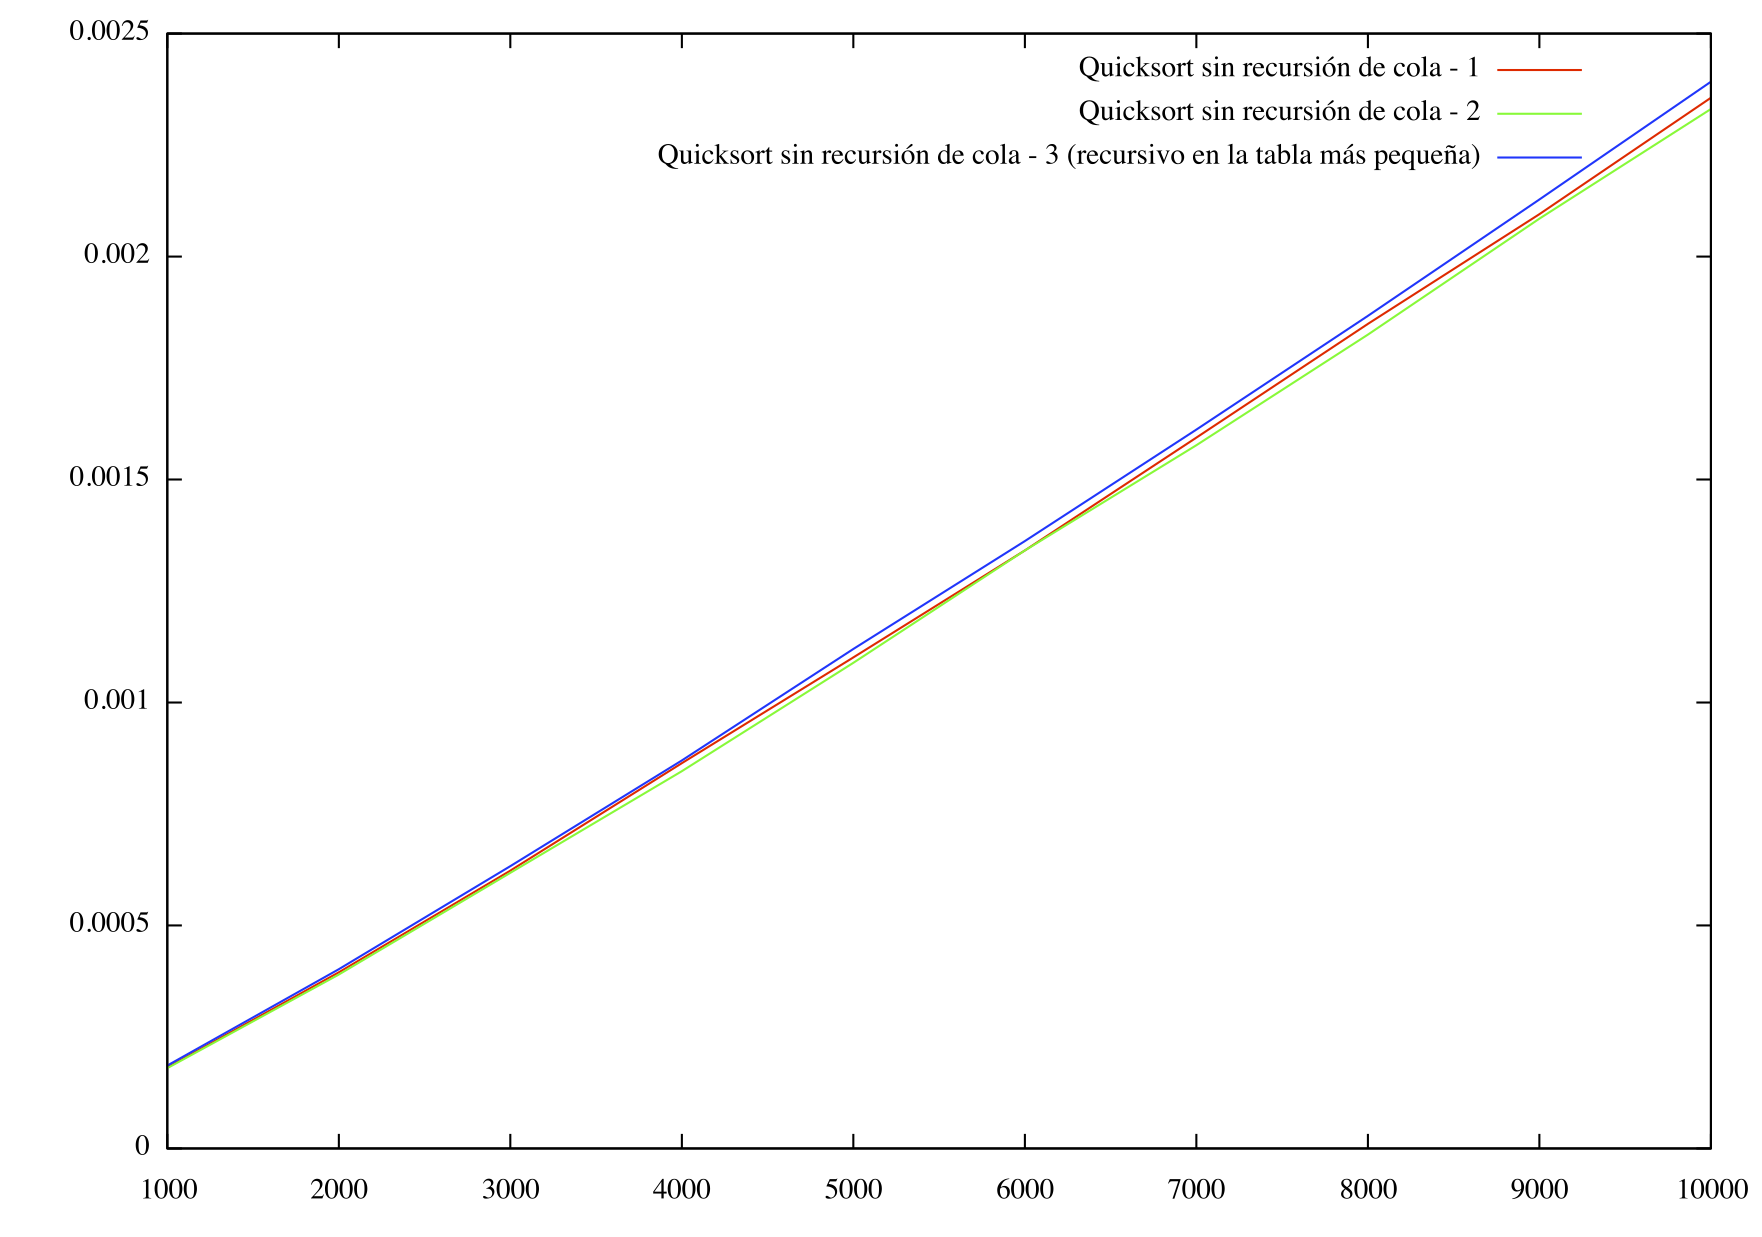
\includegraphics[width = 0.8\textwidth]{Grafica.png}
\caption{Tiempo de ejecución.}
\label{fig:TiempoEjecucion}
\end{figure}

Hemos comprobado que el código de nuestra función \texttt{quick\_sort} ordena correctamente cualquier permutación aleatoria de números\footnote{El tamaño máximo probado ha sido de 10.000 elementos.}.
Además, hemos comprobado su rendimiento y hemos sacado la gráfica de resultados en la figura \ref{fig:TiempoEjecucion}. En el apéndice \ref{sec:Apendice} se pueden ver las tablas de resultados.

\section{Cuestiones}

\paragraph{\textcolor{green!30!black}{¿Cuál es la complejidad algorítmica de QuickSort?}} La complejidad de QuickSort está dada por la fórmula de recurrencia de \eqref{eq:QuickSort}.

\begin{equation}
T(n) = \mathcal{O}(n) + 2 T \left(\frac{n}{2}\right) \implies T(n) = \mathcal{O}(n \log n)
\label{eq:QuickSort}
\end{equation}

\vspace{10pt} % Un poco de espacio adicional para separar la línea
\hrule

\paragraph{\textcolor{green!30!black}{¿Cuál es el peor caso de QuickSort?}}
El peor caso ocurre con listas ordenadas, en cuyo caso el tiempo de ejecución es $\mathcal{O}(n^2)$.

\clearpage % Forzamos a que el apéndice aparezca en una página nueva
\appendix
\section{Tablas de resultados}
\label{sec:Apendice}

\begin{table}[hbtp]
\centering
\begin{tabular}{c|cc}
\toprule % Toprule, midrule y bottomrule vienen del paquete booktabs
\textbf{Tamaño} & \textbf{Tiempo de ejecución} & \textbf{Comparaciones medias} \\ \midrule
5000 & 0.001082 & 71981.35 \\
5010 & 0.001091 & 71255.25 \\
5020 & 0.001087 & 72329.20 \\
5030 & 0.001079 & 70837.25 \\
5040 & 0.001093 & 72197.30 \\
5050 & 0.001080 & 71829.80 \\
5060 & 0.001080 & 72027.25 \\ \bottomrule
\end{tabular}
\caption{Algunos tiempos de ejecución de QuickSort.}
\label{tab:QuickSort}
\end{table}


\end{document}
